\subsection{Image Formation and Camera Models}

Each depth sensors measurement returns a matrix with depth or range values.
The projection model of the sensor performs the calculation of the camera coordinates for each point.
Additionally, sensor usually experience some form of imperfection in the imaging process, like lense distortion or misalignment of components.
These imperfections are corrected with additional models, like the distortion model for pinhole cameras.

Both calibration and error correction are out of the scope of this thesis and sensor input is expected to adhere to the basic models.
This might require preprocessing of the raw sensor data.
On robotic platforms like \acrlong{ROS} this is done automatically when providing a matching calibration of the sensor.

\subsubsection{Pinhole Camera Model}

The pinhole camera model is the most common camera model in computer vision modelling both classical and depth cameras.

\begin{figure}[H]
    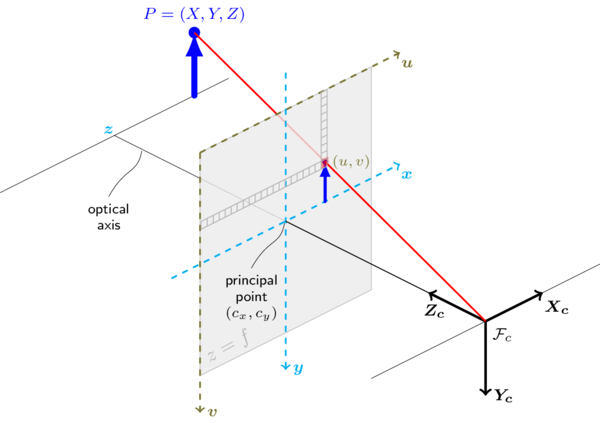
\includegraphics[width=0.6\textwidth]{chapter03/img/pinhole_camera_model.png}
    \caption[Pinhole Camera Model]{The pinhole camera model performs the perspective projection of three dimensional points into the plane. Real cameras additionally have a lense system that can result in radial and tangential distortion. These effects must be componsenated with a proper calibration of distortion models. The camera-coordinate-to-pixel-coordinate projection looses information on the depth. Therefore, the back projection results only in the direction of the light ray. The depth sensor gives the additional distance information to recover the point in camera coordinates. Graphic adopted from\cite{opencv_pinhole}.}\label{fig:pinhole_model}
\end{figure}
Figure~\ref{fig:pinhole_model} shows the perspective projection of three-dimensional points onto the plane.
This projection reduces the input dimension by one and is not depth preserving.

The model is parameterized by the focal length $f_x$ and $f_y$ that correspond to the distance of the pinhole to the image plane, the skew $s$ that resembles non-quadratic pixel shape and is most of the time $s = 0$ and the image center $c_x$ and $c_y$.

\subsubsection*{Forward Projection}

Let $\vec{P} = \rowvecxxx{X}{Y}{Z}$ be a world point in camera coordinates.
The perspective projection
\begin{equation}
    \vec{\hat{p}} = \colvecxxx{x}{y}{1} = \frac{1}{Z}\colvecxxx{X}{Y}{Z}
    \label{eq:pinhole_forward}
\end{equation}
results in the point $\vec{P}$ in image coordinates $\vec{\hat{p}}$. This step looses the depth information.
The image coordinates could be distorted and any correction would happen at this stage.
Multiplication of the $3 \times 3$ camera matrix $K$ and the homogeneous image coordinates results in the final pixel coordinates.
\begin{equation}
\begin{aligned}
K &= \begin{pmatrix}
        f_x & f_x s & c_x \\
        0   & f_y   & c_y \\
        0   & 0     & 1
     \end{pmatrix} \\
K \vec{\hat{p}} &= \begin{pmatrix}
        f_x & f_x s & c_x \\
        0   & f_y   & c_y \\
        0   & 0     & 1
     \end{pmatrix}\colvecxxx{x}{y}{1} = \colvecxxx{u}{v}{1} = \vec{p}
\end{aligned}
\end{equation}

\subsubsection*{Backward Projection}

Applying the inverse transformations allows to recover the direction of the light matching a pixel $\vec{p}$.
The potentially distorted image coordinates $\vec{\hat{p}}$ are obtained with the following formula.
\begin{equation}
\begin{aligned}
    \vec{\hat{p}} = \colvecxxx{x}{y}{1} &= K^{-1} \vec{p} \\
    \colvecxx{x}{y} &= \begin{pmatrix}\frac{1}{f_x} & -\frac{s}{f_y} \\ 0 & \frac{1}{f_y}\end{pmatrix} \colvecxx{u - c_x}{v - c_y}
\end{aligned}
\end{equation}
Again, if a distortion model is used, the inverse transformation needs to be applied to $\vec{\hat{p}}$.

The final step is the projection to the unit sphere that gives the direction vector of the light ray equivalent to norming the vector $\vec{\hat{p}}$.
\begin{equation}
    \colvecxxx{Xs}{Ys}{Zs} = \frac{1}{\sqrt{x^2 + y^2 + 1}} \colvecxxx{x}{y}{1}
    \label{eq:pinhole_backward}
\end{equation}

\subsubsection{Equirectangular Camera Model}

The equirectangular camera model maps the whole unit sphere to the plane.
Equirectangular images have constant, but potentially different angular resolution in $x$- and $y$-direction.
This mapping stores panoramas that are usually stitched together from multiple cameras.
The \acrshort{LIDAR} sensor output can be stored as an equirectangular image as well.
Supporting this camera model gives flexibility to support all kind of sensors as multiple pinhole sensors can be stitched to one virtual sensor and mapped to the equirectangular model.

\begin{figure}[H]
    \scalebox{0.9}{%
    

% Gradient Info
  
\tikzset {_5hbmo8yc4/.code = {\pgfsetadditionalshadetransform{ \pgftransformshift{\pgfpoint{81.84 bp } { -103.62 bp }  }  \pgftransformscale{1.32 }  }}}
\pgfdeclareradialshading{_42co7mn6x}{\pgfpoint{-72bp}{88bp}}{rgb(0bp)=(1,1,1);
rgb(0.052081516810825894bp)=(1,1,1);
rgb(25bp)=(0.74,0.74,0.74);
rgb(400bp)=(0.74,0.74,0.74)}
\tikzset{every picture/.style={line width=0.75pt}} %set default line width to 0.75pt        

\begin{tikzpicture}[x=0.75pt,y=0.75pt,yscale=-1,xscale=1,style = {font = \boldmath}]
%uncomment if require: \path (0,313); %set diagram left start at 0, and has height of 313

%Shape: Circle [id:dp5460928729364494] 
\draw  [draw opacity=0][shading=_42co7mn6x,_5hbmo8yc4][line width=1.5]  (24,163.5) .. controls (24,96.4) and (78.4,42) .. (145.5,42) .. controls (212.6,42) and (267,96.4) .. (267,163.5) .. controls (267,230.6) and (212.6,285) .. (145.5,285) .. controls (78.4,285) and (24,230.6) .. (24,163.5) -- cycle ;
%Straight Lines [id:da5671603358142259] 
\draw [color={rgb, 255:red, 74; green, 74; blue, 74 }  ,draw opacity=1 ] [dash pattern={on 4.5pt off 4.5pt}]  (145.5,163.5) -- (202,187.33) ;
%Shape: Ellipse [id:dp6506733150555541] 
\draw  [color={rgb, 255:red, 74; green, 74; blue, 74 }  ,draw opacity=1 ][dash pattern={on 4.5pt off 4.5pt}] (76,163.5) .. controls (76,96.4) and (107.12,42) .. (145.5,42) .. controls (183.88,42) and (215,96.4) .. (215,163.5) .. controls (215,230.6) and (183.88,285) .. (145.5,285) .. controls (107.12,285) and (76,230.6) .. (76,163.5) -- cycle ;
%Shape: Ellipse [id:dp26678317589757317] 
\draw  [color={rgb, 255:red, 74; green, 74; blue, 74 }  ,draw opacity=1 ][dash pattern={on 4.5pt off 4.5pt}][line width=0.75]  (24,163.5) .. controls (24,143.62) and (78.4,127.5) .. (145.5,127.5) .. controls (212.6,127.5) and (267,143.62) .. (267,163.5) .. controls (267,183.38) and (212.6,199.5) .. (145.5,199.5) .. controls (78.4,199.5) and (24,183.38) .. (24,163.5) -- cycle ;
%Straight Lines [id:da95744507209868] 
\draw [line width=2.25]    (145.5,163.5) -- (305.8,163.5) ;
\draw [shift={(310.8,163.5)}, rotate = 180] [fill={rgb, 255:red, 0; green, 0; blue, 0 }  ][line width=0.08]  [draw opacity=0] (14.29,-6.86) -- (0,0) -- (14.29,6.86) -- cycle    ;
%Straight Lines [id:da9220607301798066] 
\draw [color={rgb, 255:red, 74; green, 74; blue, 74 }  ,draw opacity=1 ] [dash pattern={on 4.5pt off 4.5pt}]  (202,91) -- (202,187.33) ;
%Shape: Arc [id:dp11613747224217108] 
\draw  [draw opacity=0][line width=1.5]  (179.38,177.98) .. controls (175.34,183.79) and (164.25,188) .. (151.5,188) .. controls (141.03,188) and (132.07,185.16) .. (127.41,180.92) -- (152.5,173.67) -- cycle ; \draw  [color={rgb, 255:red, 144; green, 19; blue, 254 }  ,draw opacity=1 ][line width=1.5]  (179.38,177.98) .. controls (175.34,183.79) and (164.25,188) .. (151.5,188) .. controls (141.03,188) and (132.07,185.16) .. (127.41,180.92) ;
%Shape: Arc [id:dp1998195952216596] 
\draw  [draw opacity=0][line width=1.5]  (166.45,136.09) .. controls (175.38,141.4) and (181.85,150.81) .. (182.82,161.52) .. controls (183.36,167.6) and (182.07,173.26) .. (179.38,177.98) -- (152.82,161.52) -- cycle ; \draw  [color={rgb, 255:red, 245; green, 166; blue, 35 }  ,draw opacity=1 ][line width=1.5]  (166.45,136.09) .. controls (175.38,141.4) and (181.85,150.81) .. (182.82,161.52) .. controls (183.36,167.6) and (182.07,173.26) .. (179.38,177.98) ;
%Straight Lines [id:da3798410950733011] 
\draw [color={rgb, 255:red, 65; green, 117; blue, 5 }  ,draw opacity=1 ][line width=1.5]    (145.5,163.5) -- (199.07,93.67) ;
\draw [shift={(201.5,90.5)}, rotate = 487.49] [fill={rgb, 255:red, 65; green, 117; blue, 5 }  ,fill opacity=1 ][line width=0.08]  [draw opacity=0] (11.61,-5.58) -- (0,0) -- (11.61,5.58) -- cycle    ;
%Shape: Circle [id:dp5016585286703897] 
\draw  [draw opacity=0][fill={rgb, 255:red, 74; green, 144; blue, 226 }  ,fill opacity=1 ] (198,91) .. controls (198,88.79) and (199.79,87) .. (202,87) .. controls (204.21,87) and (206,88.79) .. (206,91) .. controls (206,93.21) and (204.21,95) .. (202,95) .. controls (199.79,95) and (198,93.21) .. (198,91) -- cycle ;
%Straight Lines [id:da5083339397538952] 
\draw [line width=2.25]    (145.5,163.5) -- (96.54,212.46) ;
\draw [shift={(93,216)}, rotate = 315] [fill={rgb, 255:red, 0; green, 0; blue, 0 }  ][line width=0.08]  [draw opacity=0] (14.29,-6.86) -- (0,0) -- (14.29,6.86) -- cycle    ;
%Straight Lines [id:da9550893076013829] 
\draw [line width=2.25]    (145.5,163.5) -- (145.5,9.47) ;
\draw [shift={(145.5,4.47)}, rotate = 450] [fill={rgb, 255:red, 0; green, 0; blue, 0 }  ][line width=0.08]  [draw opacity=0] (14.29,-6.86) -- (0,0) -- (14.29,6.86) -- cycle    ;
%Shape: Circle [id:dp9507399492507013] 
\draw  [line width=1.5]  (24,163.5) .. controls (24,96.4) and (78.4,42) .. (145.5,42) .. controls (212.6,42) and (267,96.4) .. (267,163.5) .. controls (267,230.6) and (212.6,285) .. (145.5,285) .. controls (78.4,285) and (24,230.6) .. (24,163.5) -- cycle ;

% Text Node
\draw (168,107) node [anchor=north west][inner sep=0.75pt]  [color={rgb, 255:red, 65; green, 117; blue, 5 }  ,opacity=1 ] [align=left] {$\displaystyle \mathbf{r}$};
% Text Node
\draw (156.29,184.75) node [anchor=south east] [inner sep=0.75pt]  [color={rgb, 255:red, 144; green, 19; blue, 254 }  ,opacity=1 ] [align=left] {$\displaystyle \mathbf{\varphi }$};
% Text Node
\draw (160.5,145.5) node [anchor=north west][inner sep=0.75pt]  [color={rgb, 255:red, 245; green, 166; blue, 35 }  ,opacity=1 ] [align=left] {$\displaystyle \mathbf{\theta }$};


\end{tikzpicture}

    }
    \caption[Spherical Camera Model and Equirectangular Images]{Each cartesian point that is not the origin can be uniquely converted to spherical coordinates. The origin $\mathbf{O}$ is interpreted as an invalid measurement in the context of this thesis and therefore filtered out during processing.}\label{fig:spherical}
\end{figure}

The projections are mostly a conversion from cartesian to spherical coordinates and described here in brief.
Additionally, to suite the \acrshort{LIDAR} sensor better a slight addition for a vertical field of view is added.
This field of view simply crops the full equirectangular image to the predefined slice and discards other coordinates as invalid.
Figure~\ref{fig:spherical} shows the relationship between points in spherical coordinates and the equirectangular projection.

The model is parametrized by the width $w$ and height $h$ of the image and the vertical field of view $[\theta_{min}, \theta_{max}]$ which defaults to $\theta_{min} = 0$ and $\theta_{max} = \pi$.
This definition yields the vertical and horizontal angular resolution of a pixel, which is a constant.
\begin{equation}
\label{eq:equi_angular_resolution}
\begin{aligned}
    d\varphi &= \frac{2 \pi}{w} \\
    d\theta &= \frac{\theta_{max} - \theta_{min}}{h} \\
\end{aligned}
\end{equation}
The used spherical coordinates $z = (r, \varphi, \theta)$ convention defines the radius $r \in \mathbb{R}$, the azimuthal angle $\varphi \in [-\pi, \pi)$ and the polar angle $\theta \in [0, \pi]$.
Measurements with $r = 0$ are filtered out as invalid data points.

\subsubsection*{Forward Projection}

Let $\vec{P} = \rowvecxxx{X}{Y}{Z}$ be a point in camera coordinates.
This point is converted to spherical coordinates.
\begin{equation}
\begin{aligned}
    r       &= \sqrt{X^2 + Y^2 + Z^2} \\
    \theta  &= \arccos{\frac{Z}{r}} \\
    \varphi &= \arctantwo{\frac{Y}{X}}
\end{aligned}
\end{equation}
This conversion is ill defined for $r = 0$ which corresponds to a missing range measurement and can be skipped safely.
Finally, the spherical coordinates are converted to pixel coordinates with
\begin{equation}
\begin{aligned} 
    \colvecxx{u}{v} = \colvecxx{\frac{\varphi + \pi}{d\varphi}}{\frac{\theta}{d\theta}}
\end{aligned}
\end{equation}

\subsubsection*{Backward Projection}

The backward projection recovers the light ray direction from pixel coordinates.
It is analogous to the forward projection mainly a conversion from spherical to cartesian coordinates.
Note, that $r = 1$ as the resulting vector is of unit length.
\begin{equation}
\begin{aligned}
    \varphi &= u d\varphi - \pi \\
    \theta &= \theta_{min} + v d\theta \\
    \colvecxxx{X_s}{Y_s}{Z_s} &= \colvecxxx{\sin \theta \cos \varphi}{\sin \theta \sin \varphi}{\cos \theta}
\end{aligned}
\end{equation}

\subsubsection{Range and Depth Conversion}\label{sec:range_depth_conversion}

\begin{figure}[H]
    \scalebox{0.8}{%
    

\tikzset{every picture/.style={line width=0.75pt}} %set default line width to 0.75pt        

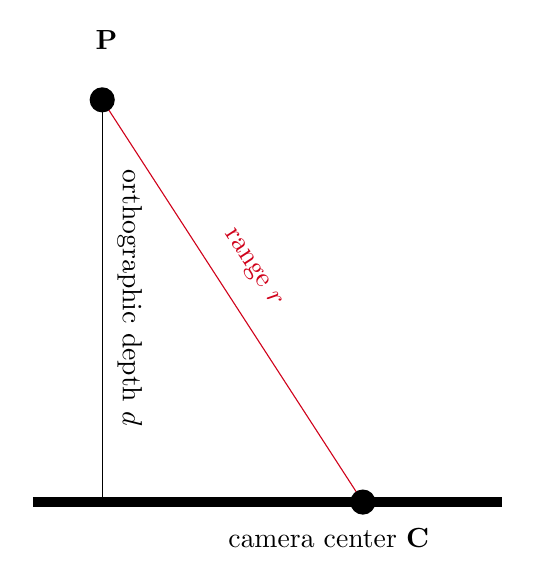
\begin{tikzpicture}[x=0.75pt,y=0.75pt,yscale=-1,xscale=1]
%uncomment if require: \path (0,273); %set diagram left start at 0, and has height of 273

%Straight Lines [id:da7423207506186664] 
\draw [line width=3.75]    (17.08,234.29) -- (243.08,234.29) ;
%Straight Lines [id:da2664879119929795] 
\draw    (50.5,40.5) -- (50.5,234.92) ;
%Straight Lines [id:da2932541940464021] 
\draw [color={rgb, 255:red, 208; green, 2; blue, 27 }  ,draw opacity=1 ]   (50.5,40.5) -- (176.08,234.29) ;
%Shape: Circle [id:dp5274939901831479] 
\draw  [draw opacity=0][fill={rgb, 255:red, 0; green, 0; blue, 0 }  ,fill opacity=1 ] (170.02,234.29) .. controls (170.02,230.94) and (172.74,228.23) .. (176.08,228.23) .. controls (179.43,228.23) and (182.15,230.94) .. (182.15,234.29) .. controls (182.15,237.64) and (179.43,240.35) .. (176.08,240.35) .. controls (172.74,240.35) and (170.02,237.64) .. (170.02,234.29) -- cycle ;
%Shape: Circle [id:dp5178837685841811] 
\draw  [draw opacity=0][fill={rgb, 255:red, 0; green, 0; blue, 0 }  ,fill opacity=1 ] (44.44,40.5) .. controls (44.44,37.15) and (47.15,34.44) .. (50.5,34.44) .. controls (53.85,34.44) and (56.56,37.15) .. (56.56,40.5) .. controls (56.56,43.85) and (53.85,46.56) .. (50.5,46.56) .. controls (47.15,46.56) and (44.44,43.85) .. (44.44,40.5) -- cycle ;

% Text Node
\draw (114.53,100) node [anchor=north west][inner sep=0.75pt]  [color={rgb, 255:red, 208; green, 2; blue, 27 }  ,opacity=1 ,rotate=-56.88] [align=left] {range $\displaystyle r$};
% Text Node
\draw (71,73) node [anchor=north west][inner sep=0.75pt]  [rotate=-90] [align=left] {orthographic depth $\displaystyle d$};
% Text Node
\draw (110,246) node [anchor=north west][inner sep=0.75pt]  [color={rgb, 255:red, 0; green, 0; blue, 0 }  ,opacity=1 ] [align=left] {camera center $\displaystyle \mathbf{C}$};
% Text Node
\draw (46,6) node [anchor=north west][inner sep=0.75pt]   [align=left] {$\displaystyle \mathbf{P}$};


\end{tikzpicture}


    }
    \caption[Orthographic Depth and Range visualized]{The distance information of a point relative to the center of a sensor at $\vec{C}$ can either be stored as the orthographic depth, mathematically the $Z$ component of the camera coordinates or the range, equivalent to the $L2$ norm of the point $\vec{P}$ in camera coordinates. The orthographic depth is commonly provided by depth cameras and the range by \acrshort{LIDAR} systems.}
    \label{fig:range_depth}
\end{figure}

There are two possible conventions on how to store depth data, both demonstrated in Figure~\ref{fig:range_depth}.
The orthographic depth~$d$ is the distance from the image plane and commonly returned by pinhole depth sensors like the Kinectv2.
On the other hand, the range~$r$ is the $L2$ norm of the vector from the camera origin to $\vec{P}$.
For consistency and generality, depth data is converted to range data before further processing takes place.
This simplifies later conversion and mixing of different camera models in a coherent fashion.
The conversion depends on the camera model and only the pinhole model is subject to analysis here.

From the forward projection function in Equation~\ref{eq:pinhole_forward} of the pinhole model follows the connection of the range and orthographic depth of the camera coordinates $\vec{P}$ and image coordinates $\vec{\hat{p}}$ of the point $\mathbf{P}$.
\begin{equation}
\begin{aligned}
    \vec{\hat{p}} &= \colvecxxx{x}{y}{1} = \frac{1}{Z}\colvecxxx{X}{Y}{Z} \\
    \implies Z \vec{\hat{p}} &= \vec{P} \\
    \implies Z \lnorm{\vec{\hat{p}}} &= \lnorm{\vec{P}} \\
    \iff Z r &= d
\end{aligned}
\end{equation}
The inverse of the $Z_{s}$ component of the backward projection from Equation~\ref{eq:pinhole_backward} provides the scaling factor between orthographic depth and range.
Consequently, the range~$r$ for the depth~$d$ at image coordiantes $\rowvecxx{x}{y}$ with corresponding coordinates on the unit sphere $\rowvecxxx{X_s}{Y_s}{Z_s}$ is computed with
\begin{equation}
    r = \frac{d}{Z_s} = d \sqrt{x^2 + y^2 + 1}\text{.}
\end{equation}
